\subsubsection{Modellentwicklung am Objekt}
Nachdem das Testmodell (vgl. Abbildung \ref{fig:print-case-test_04}) nicht zu 100 \% gepasst hat, hat Manuel Starz die Abmessungen neu geklärt und diese in Fusion 360 übertragen (vgl. \ref{case_footprint}). Um Material für den 3D-Druck zu sparen, wurde die Zeichnung dann im Maßstab 1:1 auf Papier gedruckt, ausgeschnitten und angelegt.\par
Da hier einige Maße noch nicht gestimmt haben, hat Manuel Starz den Plan überarbeitet (vgl. \ref{case_footprint_final}). Diese neuen Bemaßungen waren dann korrekt.\par
Daraufhin wurde dann die Zeichnung in zwei eigenständige Dateien gesplittet, um die linke und die rechte Seite des Gehäuses zu konstruieren.\par
Die Grundabmessung des Bildschirms werden in Fusion 360 als neue Zeichnung angelegt. Hierzu wurde ein einfaches Rechteck mit den entsprechenden Außenmaßen angelegt (vlg. \ref{fig:design-case-01}). Anschließend wurden die Ecken mit einem Radius von 7mm abgerundet. (vgl. \ref{fig:design-case-02}). Abschließend wurde die Zeichnung in der Mitte geteilt, um die beiden Hälften des Gehäuses unabhängig
\begin{figure}[h!tb]
	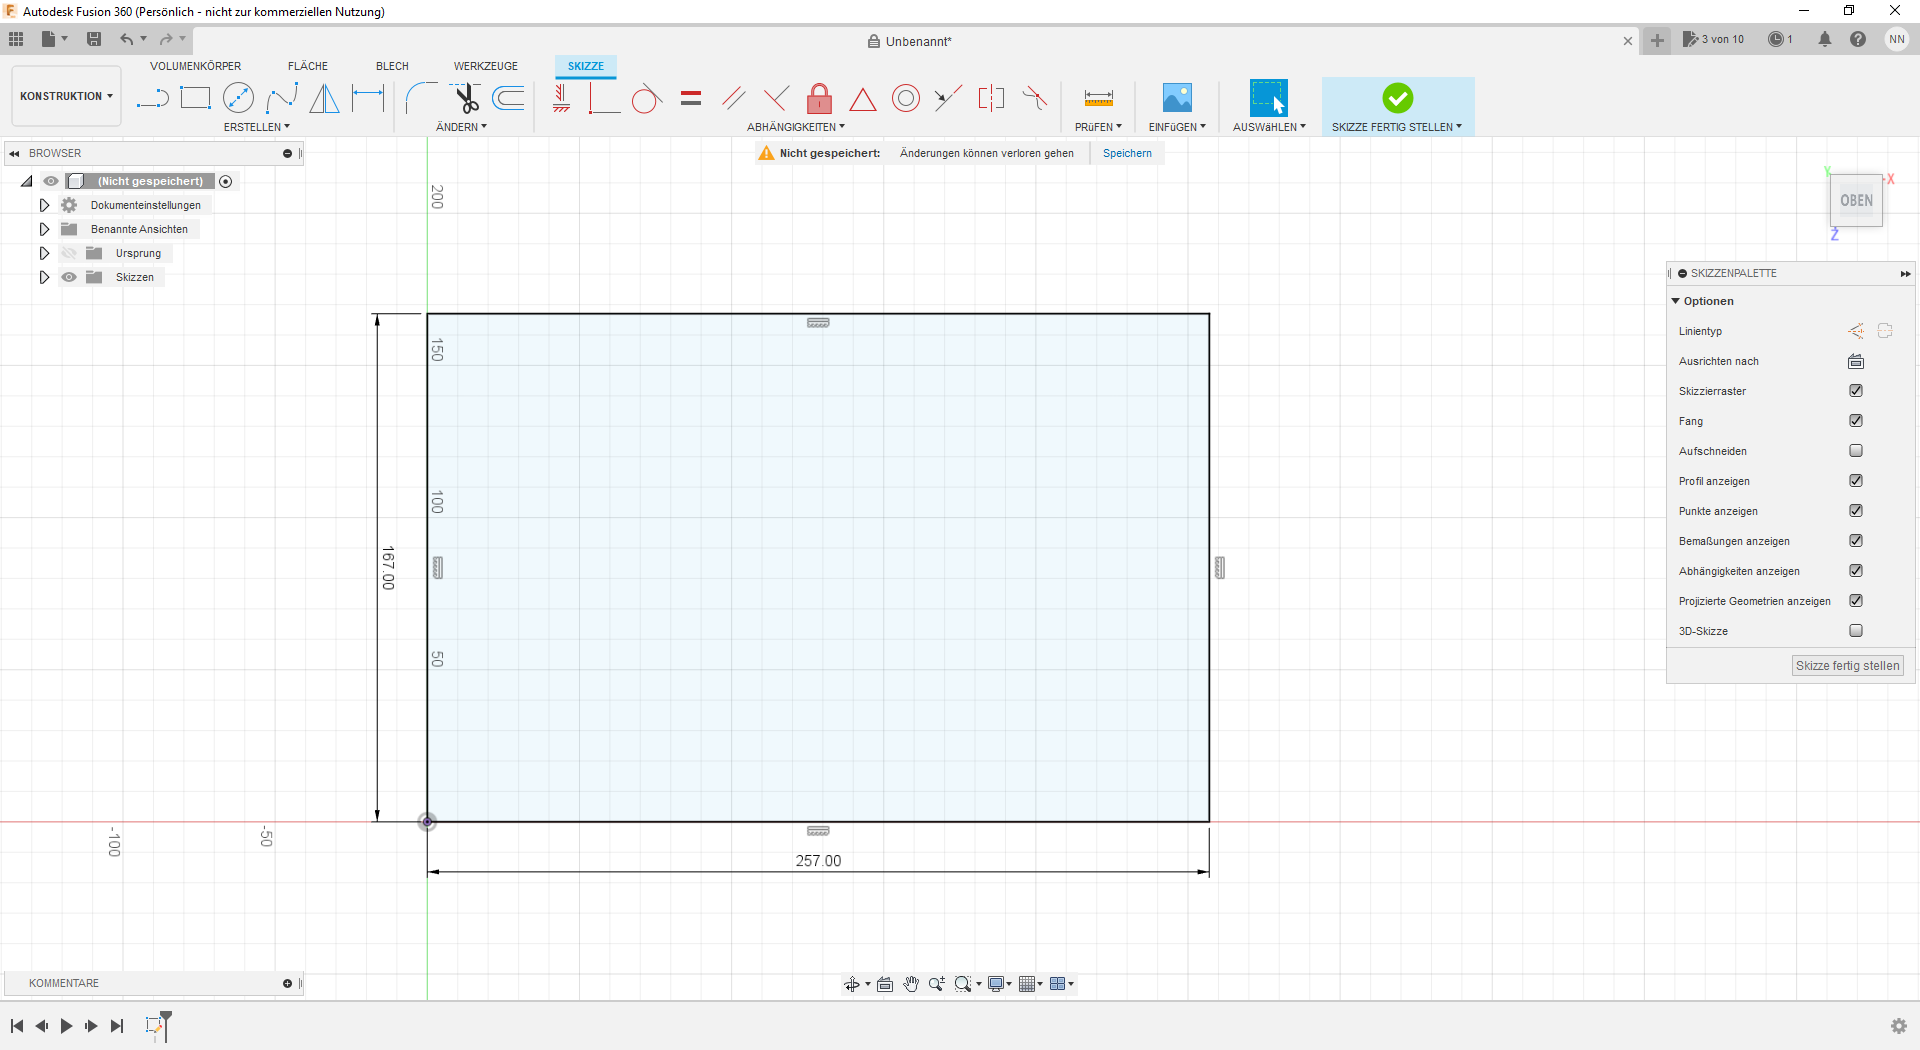
\includegraphics[width=1\textwidth]{img/konstruktion_gehaeuse_001.png}
	\caption[Zeichnen der Außenmaße]{Zeichnen der Außenmaße}
	\label{fig:design-case-01}
\end{figure}
\begin{figure}[h!tb]
	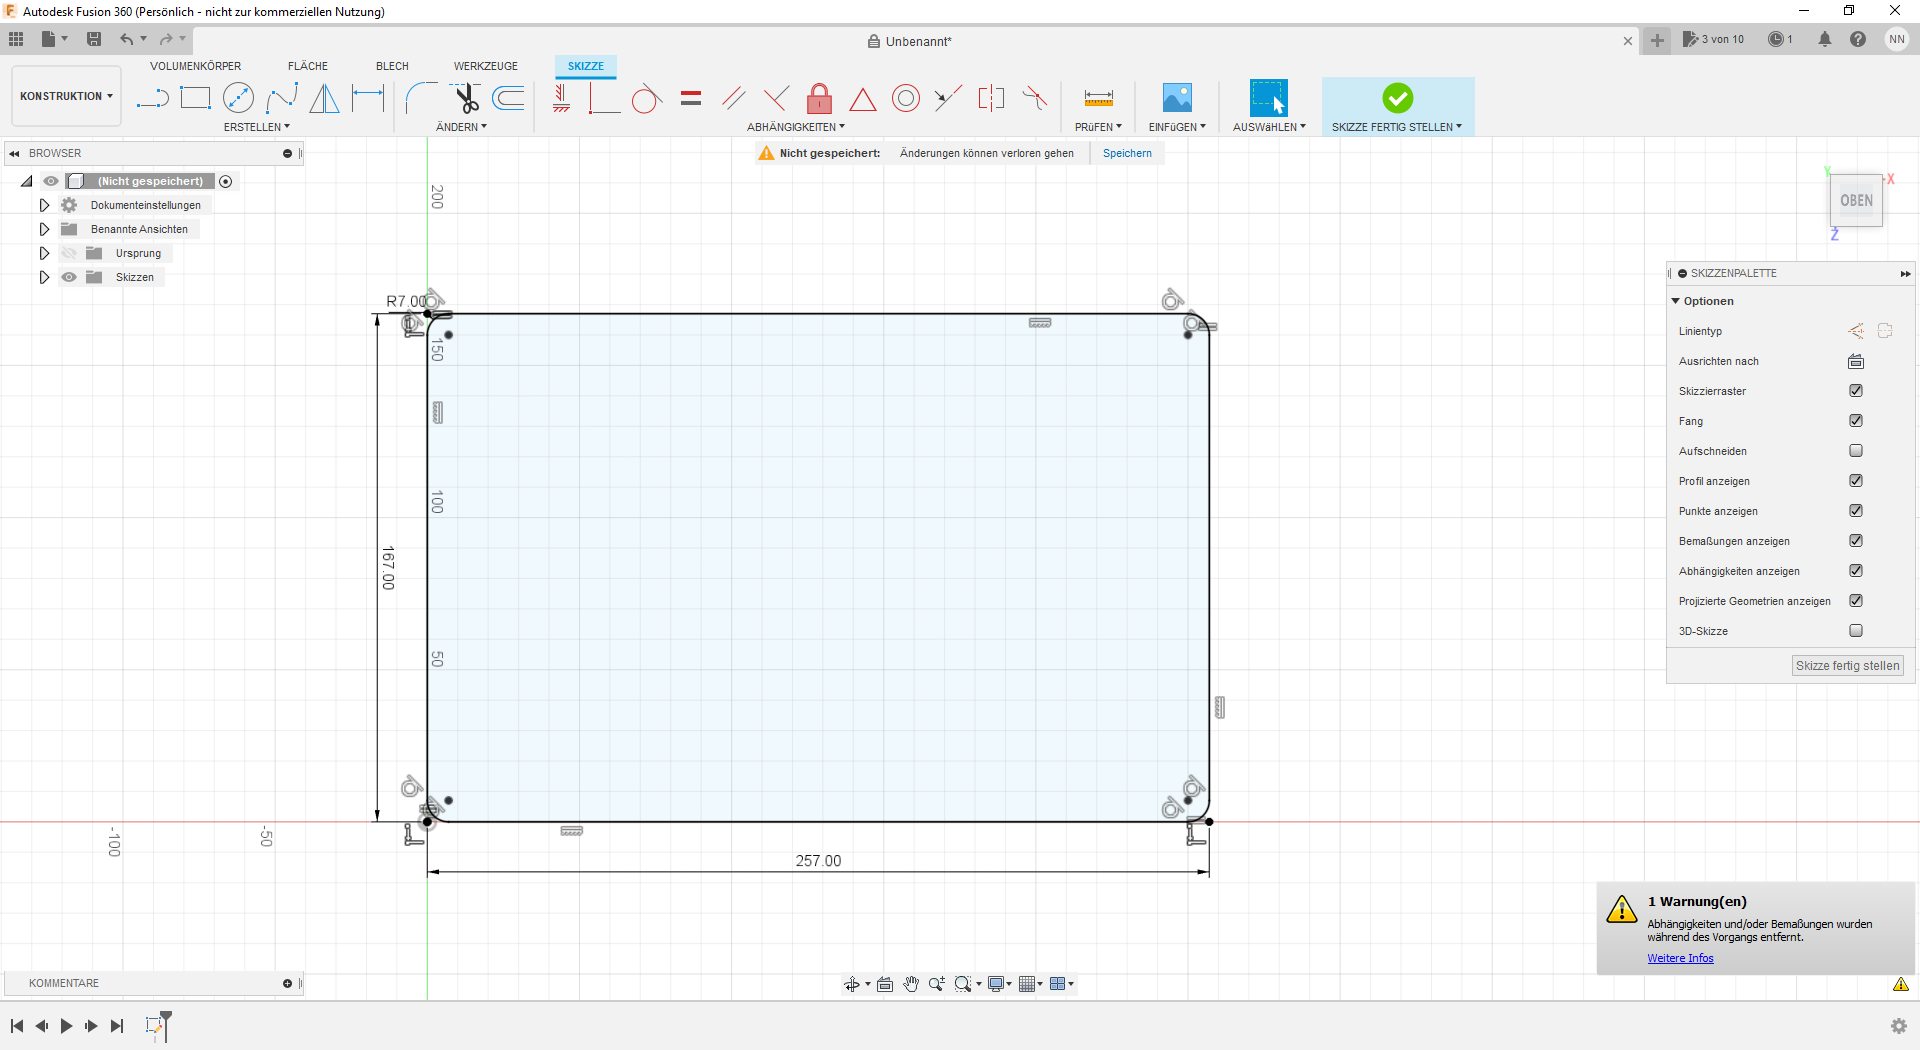
\includegraphics[width=1\textwidth]{img/konstruktion_gehaeuse_002.png}
	\caption[Abrunden der Ecken]{Abrunden der Ecken}
	\label{fig:design-case-02}
\end{figure}